
\svnid{$Id: $}
\svnid{$URL: $}

\section{FOR REVIEW:Create test case for rectangular profiles (flow area)}
\newrefsegment

%---------------------------------------------------------------------------------
\section*{Quality Assurance}
\begin{tabular}{@{}p{27mm}@{}p{0mm}p{\textwidth-52mm-48pt}p{15mm}p{10mm}}
\textbf{Date} & \textbf{:} &  October 22, 2019   \\ 
\textbf{Author} & \textbf{:} & Eskedar Gebremedhin  & \textbf{Initials:} & EG \\
\textbf{Review} & \textbf{:} &   & \textbf{Initials:} & \ldots 
\end{tabular}

%---------------------------------------------------------------------------------
\section*{Version information}
{{
\begin{tabular}{@{}p{27mm}@{}p{0mm}p{\textwidth-27mm-24pt}}
\textbf{Executable}   & \textbf{:} & Deltares, D-Flow FM Version 1.2.76.65238M, October 22, 25:48:09  \\
\textbf{Location input}     & \textbf{:} & \url{https://repos.deltares.nl/repos/DSCTestbench/trunk/cases/e02_dflowfm/f105_cross-sections/c04_rectangle-profile} \\
\textbf{Revision input} & \textbf{:} & - \\
\textbf{Location output}     & \textbf{:} & \url{https://repos.deltares.nl/repos/DSCTestbench/trunk/references/win64/e02_dflowfm/f105_cross-sections/c04_rectangle-profile} \\
\textbf{Revision output} & \textbf{:} & -
\end{tabular}
}}

%---------------------------------------------------------------------------------
\section*{Purpose}
The purpose of this validation test is to verify that D-Flow FM gives the correct result with the implementation of rectangular profiles and that upstream water depth/water level shows the right balance between roughness and resistance while applying different roughness types.

%---------------------------------------------------------------------------------
\section*{Linked claims}
\begin{enumerate}
\item \dflowfm can take into account the shape of several cross sectional profiles (rectangle, rectangle, ZW, XYZ and YZ).
\item \dflowfm can accurately simulate steady and unsteady hydrostatic flow on 1D networks.
\end{enumerate}
%---------------------------------------------------------------------------------
\section*{Approach}
Rectangular profiles are validated for different roughness types by verifying that the upstream water depth of the channels reaches the correct value under steady state forcing. 
The model consist of 9 sub-models T1 to T9, each sub-model is parametrized with the same rectangular profile and longitudinal slope but with different roughness values (and types) per sub-model.
For each sub-model, the equilibrium upstream conveyance $K(h)$ at equilibrium is analytically computed for a constant water depth ($h$) of 1.5 m using the equations for rectangular flow area described in \autoref{10405:description of flowing less than half full rectangular cross-section}.
The calculated conveyance is converted to constant upstream discharge boundary ($Q$) condition using the equation $Q=K\sqrt{S}$ where $S$ is the slope of the channel. 

To verify the claims, the modelled (upstream) water depth and water level should equal 1.5 m and 6.5 m AD, respectively. 

%---------------------------------------------------------------------------------
\section*{Conclusion} 
The implementation of rectangular profile for steady state simulations while applying a downstream water level boundary close to equilibrium depth is considered to be satisfactory. 
This conclusion is valid for the application of the following roughness coefficients:

\begin{itemize}
\item Ch\'ezy
\item Manning
\item Strickler ks
\item Nikuradse (Strickler)
\item Nikuradse (White \& Colebrook) 
\item De Bos \& Bijkerk
\end{itemize}

\dflowfm modelled water level and water depth match the analytical solution in all sub-models. 
The result also supports the claim that the boundary conditions (constant) are properly applied. 


%---------------------------------------------------------------------------------
\section*{Model description}
The test comprises of nine separate sub-models T1 to T9 (see \autoref{fig:e02_f105_c04_layout}). 
The models are 20 km in length and have an equidistant grid spacing of dx=50 m; flow is from right (x=20000) to left (x=0). A 4 m width and height of rectangular profile applied at the downstream end (x=0) for each sub-model. The rectangular profile at x=20000 is shifted with 5 m up relative to the rectangular profile at x=0. 
Consequently, bed level decreases from 5 m at x=20000 (East, upstream) to 0 m at x=0 (West, downstream) resulting in a slope of 1.5e-4. 

The boundary conditions of each sub-model is listed in \autoref{tab:e02_f105_c04_BC}. 
The upstream flow boundary conditions are parametrized to ensure that all sub-models are at equilibrium with a water depth of 1.5 m. The upstream boundary condition varies for each sub-model as their roughness types and values are different. 
To ensure that water depth are at 1.5 m at x=0, the downstream boundary condition is set to $1.5-(S*\frac{dx}{2})$. 
This is because water level boundaries are in \dflowfm not applied at the last grid point of the network, but depending on the setting of  \texttt{izbndpos} some distance outside the system. 
For these simulations we have set \texttt{izbndpos = 1} which means that the water levels are imposed half a computational grid cell length outside the system.


\begin{figure}[H]
\centering
\begin{subfigure}{\textwidth}
\centering
\includegraphics*[width=0.95\textwidth]{figures/e02_f105_c04_layout.png}
\caption{Overview} 
\end{subfigure}
\begin{subfigure}{.5\textwidth}
  \centering
  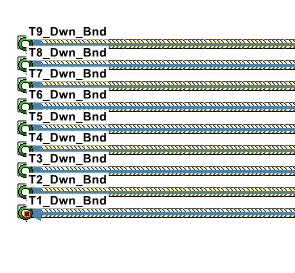
\includegraphics[width=.9\linewidth]{figures/e02_f105_c04_lay-out_zoom_dwn.PNG}
  \caption{Zoom-in at downstream end (x=0)}
\end{subfigure}%
\begin{subfigure}{.5\textwidth}
  \centering
  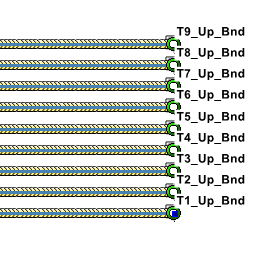
\includegraphics[width=.8\linewidth]{figures/e02_f105_c04_lay-out_zoom_up.PNG}
  \caption{Zoom-in at upstream end (x=20000)} 
\end{subfigure}
\caption{Lay-out of the test model}
\label{fig:e02_f105_c04_layout}
\end{figure}


\begin{longtable}{|p{18mm}|p{23mm}|p{30.5mm}|p{68.5mm}|}
\caption{Boundary conditions applied in sub-models T1 to T9.} 
\label{tab:e02_f105_c04_BC} \\ 
\hline 
\STRUT
      Sub-model
	 & x-coord. \unitbrackets{m} 
	 &  ID  
	 &  Boundary condition  \\ 
[1ex] \hline \endhead
\hline
\endfoot
%
\STRUT
T1 & 20000.00     & T1\_Up\_Bnd   & {Constant Discharge:  of 3.9524 m\textsuperscript{3}s\textsuperscript{-1} }   	\\
                                                & 0.00        & T1\_Dwn\_Bnd   & {Constant Water level: of 1.49375 m AD}  \\
\STRUT
T2 & 20000.00     & T2\_Up\_Bnd   & {Constant Discharge:  of 1.71206 m\textsuperscript{3}s\textsuperscript{-1} }   	  \\
                                                & 0.00        & T2\_Dwn\_Bnd   & {Constant Water level: of 1.49375 m AD}  \\
\STRUT
T3 & 20000.00     & T3\_Up\_Bnd   & {Constant Discharge:  of 3.42413 m\textsuperscript{3}s\textsuperscript{-1}  }       \\
                                               & 0.00        & T3\_Dwn\_Bnd   & {Constant Water level: of 1.49375 m AD}    \\
\STRUT											   
T4 & 20000.00     & T4\_Up\_Bnd   & {Constant Discharge:  of 2.22943 m\textsuperscript{3}s\textsuperscript{-1} }       \\
                                               & 0.00        & T4\_Dwn\_Bnd   & {Constant Water level: of 1.49375 m AD}    \\
\STRUT											   
T5 & 20000.00     & T5\_Up\_Bnd   & {Constant Discharge:  of 2.42695 m\textsuperscript{3}s\textsuperscript{-1}}         \\
                                                & 0.00        & T5\_Dwn\_Bnd   & {Constant Water level: of 1.49375 m AD}    \\
\STRUT											   
T6  & 20000.00     & T6\_Up\_Bnd   & {Constant Discharge:  of 3.14121 m\textsuperscript{3}s\textsuperscript{-1}}       \\
                                                & 0.00        & T6\_Dwn\_Bnd   & {Constant Water level: of 1.49375 m AD}  \\
\STRUT
T7  & 20000.00     & T7\_Up\_Bnd   & {Constant Discharge:  of 2.93974 m\textsuperscript{3}s\textsuperscript{-1} }    \\
                                               & 0.00        & T7\_Dwn\_Bnd   & {Constant Water level: of 1.49375 m AD}  \\
\STRUT
T8 & 20000.00     & T8\_Up\_Bnd   & {Constant Discharge:  of 3.42413 m\textsuperscript{3}s\textsuperscript{-1} }      \\
                                               & 0.00        & T8\_Dwn\_Bnd   & {Constant Water level: of 1.49375 m AD} \\
\STRUT
T9  & 20000.00     & T9\_Up\_Bnd   & {Constant Discharge:  of 3.52768 m\textsuperscript{3}s\textsuperscript{-1}  }   \\
                                               & 0.00        & T9\_Dwn\_Bnd   & {Constant Water level: of 1.49375 m AD} \\ [1ex]
\end{longtable}	 

The flow area $A$ and wetted perimeter $P$ of each sub-model are calcualted based on the approach discussed in  \autoref{10405:description of flowing less than half full rectangular cross-section}. 
\autoref{tab:e02_f105_c04_Roughness} shows the roughess types and values that are used on eact sub-model. The hydraulic radius $R$ is computed using the area and wetted perimeter calculated for rectangular cross-section. 


\begin{longtable}{|p{18mm}|p{55.0mm}|p{35.0mm}|}
\caption{Roughness values of T1 to T9 of the rectangular profile.} 
\label{tab:e02_f105_c04_Roughness} \\ 
\hline 
\STRUT
     Sub-model
	 &  Roughness type 
	 &  Roughness value  \\ 
[1ex] \hline \endhead
\hline
\endfoot
%
\STRUT
T1 &  Ch\'ezy & 45 \\
\STRUT
T2 & Manning & 0.05 \\
\STRUT
T3 &  Strickler & 40 \\
\STRUT
T4 & Nikuradse (White \& Colebrook)   & 0.4 \\
\STRUT
T5 & Nikuradse (White \& Colebrook)   & 0.3 \\
\STRUT
T6 & Nikuradse (Strickler) & 0.1 \\
\STRUT
T7 & De Bos \& Bijkerk & 30 \\
\STRUT
T8 & Manning & 0.025 \\
\STRUT
T9 & De Bos \& Bijkerk & 36 \\ [1ex]
\end{longtable}

%---------------------------------------------------------------------------------
\section*{Results}
The modeled water depths along sub-models T1 to T9 are on \autoref{fig:e02_f105_c04_WaterDepthEntireLength}. 
Water level and water depth differences are shown for sub-models T1 to T9 in \autoref{tab:e02_f105_c04_WaterlevelDifference} and \autoref{tab:e02_f105_c04_WaterdepthDifference}, respectively.


\begin{figure}[H]
    \centering
    \includegraphics*[width=1.05\textwidth]{figures/e02_f105_c04_Water_Depth_EntireLength.jpg}
    \caption{Water depths along sub-models T1 to T9}
    \label{fig:e02_f105_c04_WaterDepthEntireLength}
\end{figure} 


\begin{longtable}{|p{18mm}|p{20.5mm}|p{19.5mm}|p{20.5mm}|p{35mm}|}
\caption{Upstream (x=20000) modelled and expected analytical water level ($\zeta$)}. 
\label{tab:e02_f105_c04_WaterlevelDifference}\\
\hline
\STRUT
	   Sub-model
	 & ID
	 & $\zeta$\textsubscript{modelled} \unitbrackets{m} 
	 & $\zeta$\textsubscript{analytical} \unitbrackets{m} 
	 & $\Delta\zeta$\textsubscript{modelled-analytical} \unitbrackets{m} \\ 
[1ex] \hline \endhead
\hline
\endfoot
%
\STRUT 
T1     & T1\_Up\_Bnd  & 6.50   & 6.50  &  0.00    \\
\STRUT 
T2     & T2\_Up\_Bnd  & 6.50   & 6.50  &  0.00    \\
\STRUT 
T3     & T3\_Up\_Bnd  & 6.50   & 6.50  &  0.00    \\
\STRUT 
T4     & T4\_Up\_Bnd  & 6.50   & 6.50  &  0.00    \\
\STRUT 
T5     & T5\_Up\_Bnd  & 6.50   & 6.50  &  0.00    \\
\STRUT 
T6     & T6\_Up\_Bnd  & 6.50   & 6.50  &  0.00    \\
\STRUT 
T7     & T7\_Up\_Bnd  & 6.50   & 6.50  &  0.00    \\
\STRUT 
T8     & T8\_Up\_Bnd  & 6.50   & 6.50  &  0.00    \\
\STRUT 
T9     & T9\_Up\_Bnd  & 6.50   & 6.50  &  0.00   \\ [1ex]
\end{longtable}

\newpage
\begin{longtable}{|p{18mm}|p{20.5mm}|p{19.5mm}|p{20.5mm}|p{35mm}|}
\caption{Upstream (x=20000) modelled and expected analytical water depth ($h$)} 
\label{tab:e02_f105_c04_WaterdepthDifference}\\
\hline
\STRUT
	   Sub-model
	 & ID
	 & $h$\textsubscript{modelled} \unitbrackets{m} 
	 & $h$\textsubscript{analytical} \unitbrackets{m} 
	 & $\Delta h$\textsubscript{modelled-analytical} \unitbrackets{m} \\ 
[1ex] \hline \endhead
\hline
\endfoot
%
\STRUT 
T1     & T1\_Up\_Bnd  & 1.50   & 1.50  &  0.00   \\
\STRUT                                        
T2     & T2\_Up\_Bnd  & 1.50   & 1.50  &  0.00   \\
\STRUT                                        
T3     & T3\_Up\_Bnd  & 1.50   & 1.50  &  0.00   \\
\STRUT                                        
T4     & T4\_Up\_Bnd  & 1.50   & 1.50  &  0.00   \\
\STRUT                                        
T5     & T5\_Up\_Bnd  & 1.50   & 1.50  &  0.00   \\
\STRUT                                        
T6     & T6\_Up\_Bnd  & 1.50   & 1.50  &  0.00   \\
\STRUT                                        
T7     & T7\_Up\_Bnd  & 1.50   & 1.50  &  0.00   \\
\STRUT                                        
T8     & T8\_Up\_Bnd  & 1.50   & 1.50  &  0.00   \\
\STRUT                                        
T9     & T9\_Up\_Bnd  & 1.50   & 1.50  &  0.00  \\ [1ex]
\end{longtable}


%---------------------------------------------------------------------------------
\section*{Analysis of results}
All sub-models converge to an equilibrium water depth. The modelled water levels and water depths match the analytical solutions.

\section*{Reactangular profile flow area} \label{10405:description of flowing less than half full rectangular cross-section}

The equations needed to calculate the flow area $A(h)$, the wetted perimeter, $P(h)$, and the hydraulic radius, $R(h)$ are shown below along with a figure (\autoref{fig:e02_f105_c04_rectangular_profile}) that shows the 
parameters for a rectangular cross-section. It should be noted that the parameters width $W$ and flow depth $h$ are used in the equations for $A(h)$ and $P(h)$. 


\begin{figure}[H]
    \centering
    \includegraphics*[width=0.35\textwidth]{figures/e02_f105_c04_rectangular_profile.png}
    \caption{Partially full rectangular profile}
    \label{fig:e02_f105_c04_rectangular_profile}
\end{figure} 


\[ A(h)  = Wh\]
\[ P(h) = W + 2h\]
\[ K(h) = A(h)C(h)\sqrt{R(h)}\]

where:\newline 
$\>$ $K(h)$ $\>$ Lumped conveyance at $h$ \newline 
$\>$ $A(h)$ $\>$ Cross-sectional area at $h$ \newline 
$\>$ $C(h)$ $\>$ Chézy friction value at $h$ \newline 
$\>$ $P(h)$ $\>$ Wetted Perimeter at $h$ \newline 
$\>$ $R(h)$ $\>$ Hydraulic radius at $h(R(h)=A(h)/P(h))$ \newline 

Roughness types other than Ch\'ezy will be converted to their Ch\'ezy equivalent based on the local water depth $h$ and hydraulic radius $R(h)$.

%---------------------------------------------------------------------------------
\printrefsegment
